\documentclass[12pt,titlepage]{article}
\usepackage[margin=1.25in]{geometry}
\usepackage{graphicx,amsmath,blindtext,minted}

%% Variables definition
\newcommand{\vSubject}{Data Structure and Algorithm Practicum}
\newcommand{\vSubtitle}{Binary Tree}
\newcommand{\vName}{Muhammad Baihaqi Aulia Asy'ari}
\newcommand{\vNIM}{2241720145}
\newcommand{\vClass}{1I}
\newcommand{\vDepartment}{Information Technology}
\newcommand{\vStudyProgram}{D4 Informatics Engineering}

%% [START] Tikz related stuff
\usepackage{tikz}
\usetikzlibrary{svg.path,calc,shapes.geometric,shapes.misc}
\tikzstyle{terminator} = [rectangle, draw, text centered, rounded corners = 1em, minimum height=2em]
\tikzstyle{preparation} = [chamfered rectangle, chamfered rectangle sep=0.75em, draw, text centered, minimum height = 2em]
\tikzstyle{process} = [rectangle, draw, text centered, minimum height=2em]
\tikzstyle{decision} = [diamond, aspect=2, draw, text centered, minimum height=2em]
\tikzstyle{data}=[trapezium, draw, text centered, trapezium left angle=60, trapezium right angle=120, minimum height=2em]
\tikzstyle{connector} = [line width=0.25mm,->]
%% [END] Tikz related stuff

%% [START] Fancy header related stuff
\usepackage{fancyhdr}
\pagestyle{fancy}
\setlength{\headheight}{15pt} % compensate fancyhdr style
\fancyhead{}
\fancyfoot{}
\fancyfoot[L]{\thepage}
\fancyfoot[R]{\textit{\vSubject - \vSubtitle}}
\renewcommand{\footrulewidth}{0.4pt}% default is 0pt, overline for footer
%% [END] Fancy header related stuff

%% [START] Custom tabular command related stuff
\usepackage{tabularx}
\newcommand{\details}[2]{
    #1 & #2  \\
}
%% [END] Custom tabular command related stuff

%% [START] Figure related stuff
\newcommand{\image}[3][1]{
    \begin{figure}[h]
        \centering
        \includegraphics[#1]{#2}
        \caption{#3}
        \label{#3}
    \end{figure}
}
%% [END] Figure related stuff

%%
\usepackage{pgf-umlcd}

\renewcommand{\umldrawcolor}{black}
\renewcommand{\umlfillcolor}{white}
%%

%% [BEGIN] Custom enumerator
\usepackage{enumitem}
%% [END] Custom enumerator

%% [BEGIN] Paragraph indent
\usepackage{indentfirst}
%% [END] Paragraph indent

\begin{document}
\begin{titlepage}
    \centering
    \vfill
    {\bfseries\LARGE
        \vSubject\\
        \vskip0.25cm
        \vSubtitle
    }
    \vfill
    
\includegraphics[width=6cm]{images/polinema-logo.png}
    \vfill
    {
        \textbf{Name}\\
        \vName\\
        \vskip0.5cm
        \textbf{NIM}\\
        \vNIM\\
        \vskip0.5cm
        \textbf{Class}\\
        \vClass\\
        \vskip0.5cm
        \textbf{Department}\\
        \vDepartment\\
        \vskip0.5cm
        \textbf{Study Program}\\
        \vStudyProgram
    }
\end{titlepage}

\newpage

\section{COMPETENCIES}
\begin{itemize}
    \item Students are able to understand the Binary tree model
    \item Students are able to create and declare the structure of a Binary tree algorithm.
    \item Students are able to apply and implement the Binary search tree
\end{itemize}

\section{PRACTICUM 1}
In this practicum, we will try to implement Binary search tree with basic operations, using arrays (practicum 2) and linked lists (practicum 1).
\mbox{}\\
\begin{center}
    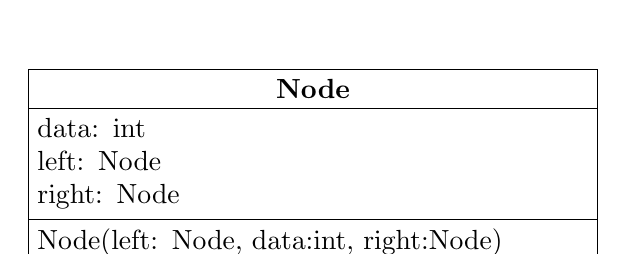
\begin{tikzpicture}
        \begin{class}[text width=7cm]{Node}{0,0}
            \attribute{data: int}
            \attribute{left: Node}
            \attribute{right: Node}
            \operation{Node(left: Node, data:int, right:Node)}
        \end{class}
    \end{tikzpicture}
\end{center}
\mbox{}\\
\begin{center}
    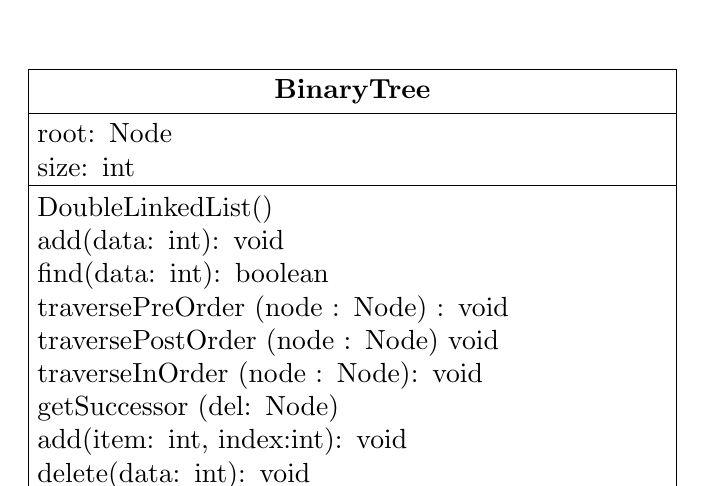
\begin{tikzpicture}
        \begin{class}[text width=8cm]{BinaryTree}{0,0}
            \attribute{root: Node}
            \attribute{size: int}
            \operation{DoubleLinkedList()}
            \operation{add(data: int): void}
            \operation{find(data: int): boolean}
            \operation{traversePreOrder (node : Node) : void}
            \operation{traversePostOrder (node : Node) void}
            \operation{traverseInOrder (node : Node): void}
            \operation{getSuccessor (del: Node)}
            \operation{add(item: int, index:int): void}
            \operation{delete(data: int): void}
        \end{class}
    \end{tikzpicture}
\end{center}
\begin{enumerate}
    \item Create \texttt{Node} , \texttt{BinaryTree} dan \texttt{BinaryTreeMain}, class
    \item In the \texttt{Node} class, add \textbf{data, left, and right} attributes as well as default and constructors with parameters
    \begin{minted}[autogobble,breaklines]{java}
        public class Node {
            int data;
            Node left;
            Node right;

            public Node() {
            }

            public Node(int data) {
                this.left = null;
                this.data = data;
                this.right = null;
            }
        }
    \end{minted}
    \item In the \texttt{BinaryTree} class, add \textbf{root} attribute.
    \begin{minted}[autogobble,breaklines]{java}
        public class BinaryTree {
            Node root;
        }
    \end{minted}
    \item Add a default constructor and the \textbf{isEmpty()} method in the \textbf{BinaryTree} class
    \begin{minted}[autogobble,breaklines]{java}
        public BinaryTree() {
            root = null;
        }

        boolean isEmpty() {
            return root==null;
        }
    \end{minted}
    \item Create \textbf{add()} method in the \textbf{BinaryTree class}. In the following image, the process of adding nodes is \textbf{not done recursively}, so that it is easier to see the process of adding nodes in a tree. Actually, if it’s done with recursive approach, the writing code will be more efficient.
    \begin{minted}[autogobble,breaklines]{java}
        void add(int data) {
            if (isEmpty()) {
                root = new Node(data);
            } else {
                Node current = root;
                while (true) {
                    if (data < current.data) {
                        if (current.left != null) {
                            current = current.left;
                        } else {
                            current.left = new Node(data);
                            break;
                        }
                    } else if (data > current.data) {
                        if (current.right != null) {
                            current = current.right;
                        } else {
                            current.right = new Node(data);
                            break;
                        }
                    } else {
                        break;
                    }
                }
            }
        }
    \end{minted}
    \item Create \textbf{find() method}
    \begin{minted}[autogobble,breaklines]{java}
        boolean find(int data) {
            boolean result = false;
            Node current = root;
            while (current != null) {
                if (current.data == data) {
                    result = true;
                    break;
                } else if (data < current.data) {
                    current = current.left;
                } else {
                    current = current.right;
                }
            }
            return result;
        }
    \end{minted}
    \item Create the \textbf{traversePreOrder(), traverseInOrder() and traversePostOrder()} methods. All of hese traverse methods are used to visit and display nodes in the tree.
    \begin{minted}[autogobble,breaklines]{java}
        void traversePreOrder(Node node) {
            if (node != null) {
                System.out.print(" " + node.data);
                traversePreOrder(node.left);
                traversePreOrder(node.right);
            }
        }

        void traversePostOrder(Node node) {
            if (node != null) {
                traversePostOrder(node.left);
                traversePostOrder(node.right);
                System.out.print(" " + node.data);
            }
        }

        void traverseInOrder(Node node) {
            if (node != null) {
                traverseInOrder(node.left);
                System.out.print(" " + node.data);
                traverseInOrder(node.right);
            }
        }
    \end{minted}
    \item Add the \textbf{getSuccessor()} method. This method will be used during the process of deleting a node that has 2 children.
    \begin{minted}[autogobble,breaklines]{java}
        Node getSuccessor(Node del) {
            Node successor = del.right;
            Node successorParent = del;
            while (successor.left != null) {
                successorParent = successor;
                successor = successor.left;
            }
            if (successor != del.right) {
                successorParent.left = successor.right;
                successor.right = del.right;
            }
            return successor;
        }
    \end{minted}
    \item Create the \textbf{delete() method}.
    \begin{minted}[autogobble,breaklines]{java}
        void delete(int data) {

        }
    \end{minted}
    In the delete method, we need to add a further validation whether the tree is empty or not. If not find the position of the node to be deleted.
    \begin{minted}[autogobble,breaklines]{java}
        if (isEmpty()) {
            System.out.println("Tree is empty");
            return;
        }

        Node parent = root;
        Node current = root;
        boolean isLeftChild = false;
        while (current != null) {
            if (current.data == data) {
                break;
            } else if (data < current.data) {
                parent = current;
                current = current.left;
                isLeftChild = true;
            } else if (data > current.data) {
                parent = current;
                current = current.right;
                isLeftChild = false;
            }
        }
    \end{minted}
    Then add the process of deleting the current node that has been found.
    \begin{minted}[autogobble,breaklines]{java}
        if (current == null) {
            System.out.println("Couldn't find data");
            return;
        } else {
            if (current.left == null && current.right == null) {
                if (current == root) {
                    root = null;
                } else {
                    if (isLeftChild) {
                        parent.left = null;
                    } else {
                        parent.right = null;
                    }
                }
            } else if (current.left == null) {
                if (current == root) {
                    root = current.right;
                } else {
                    if (isLeftChild) {
                        parent.left = current.right;
                    } else {
                        parent.right = current.right;
                    }
                }
            } else if (current.right == null) {
                if (current == root) {
                    root = current.left;
                } else {
                    if (isLeftChild) {
                        parent.left = current.left;
                    } else {
                        parent.right = current.left;
                    }
                }
            } else {
                Node successor = getSuccessor(current);
                if (current == root) {
                    root = successor;
                } else {
                    if (isLeftChild) {
                        parent.left = successor;
                    } else {
                        parent.right = successor;
                    }
                }
                successor.left = current.left;
            }
        }
    \end{minted}
    \item Open the \textbf{BinaryTreeMain} class and add the \textbf{main()} method.
    \begin{minted}[autogobble,breaklines]{java}
        public class BinaryTreeMain {
            public static void main(String[] args) {
                BinaryTree bt = new BinaryTree();

                bt.add(6);
                bt.add(4);
                bt.add(8);
                bt.add(3);
                bt.add(5);
                bt.add(7);
                bt.add(9);
                bt.add(10);
                bt.add(15);

                bt.traversePreOrder(bt.root);
                System.out.println();
                bt.traverseInOrder(bt.root);
                System.out.println();
                bt.traversePostOrder(bt.root);
                System.out.println();
                System.out.println("Find " + bt.find(5));
                bt.delete(8);
                bt.traversePreOrder(bt.root);
                System.out.println();
            }
        }
    \end{minted}
    \item Compile and run the \textbf{BinaryTreeMain} class to get more understanding of how the program tree was created.
    \item Observe the results.
\end{enumerate}

\section{PRACTICUM 2}
\begin{enumerate}
    \item In this experiment, the data tree is stored in an array and entered directly from the \textbf{main()} method, and then the traversal process is simulated in the order.
    \item Create\texttt{BinaryTreeArray} and\texttt{BinaryTreeArrayMain} class
    \item Create \textbf{data and idxLast} attributes in the \textbf{BinaryTreeArray} class. Also create \textbf{populateData () and traverseInOrder ()} methods.
    \begin{minted}[autogobble,breaklines]{java}
        public class BinaryTreeArray {
            int[] data;
            int idxLast;

            public BinaryTreeArray() {
                data = new int[10];
            }

            void populateData(int[] data, int idxLast) {
                this.data = data;
                this.idxLast = idxLast;
            }

            void traverseInOrder(int idxStart) {
                if (idxStart <= idxLast) {
                    traverseInOrder(2*idxStart+1);
                    System.out.print(data[idxStart]+" ");
                    traverseInOrder(2*idxStart+2);
                }
            }
        }
    \end{minted}
    \item Then in the \textbf{BinaryTreeArrayMain} class create the \textbf{main()} method as shown below.
    \begin{minted}[autogobble,breaklines]{java}
        public class BinaryTreeArrayMain {
            public static void main(String[] args) {
                BinaryTreeArray bta = new BinaryTreeArray();
                int[] data = {6,4,8,3,5,7,9,0,0,0};
                int idxLast = 6;
                bta.populateData(data, idxLast);
                bta.traverseInOrder(0);
            }
        }
    \end{minted}
    \item Run the BinaryTreeArrayMain class and observe the results!
\end{enumerate}

\section{QUESTIONS}
\begin{enumerate}
    \item Why the data searching process is more efficient in the Binary search tree than in ordinary binary tree?
    \mbox{}\\ \texttt{Answer:} \mbox{}\\
    because it use the devide and conque algorithm
    \item Why do we need the \textbf{Node} class? what are the \textbf{left} and \textbf{right} attributes?
    \mbox{}\\ \texttt{Answer:} \mbox{}\\
    the node class is used like in linked list, to link between data or to branch the data from node to node. left node and right node are used as a branching link from the current node.
    \item \begin{enumerate}[label=\alph*.]
        \item What are the uses of the root attribute in the \textbf{BinaryTree} class?
        \mbox{}\\ \texttt{Answer:} \mbox{}\\
        the root is used like head in linked list to be the starting point of the data structure.
        \item When the tree object was first created, what is the value of \textbf{root}?
        \mbox{}\\ \texttt{Answer:} \mbox{}\\
        it started as null.
    \end{enumerate}
    \item When the tree is still empty, and a new node is added, what process will happen?
    \mbox{}\\ \texttt{Answer:} \mbox{}\\
    it will simply add data to the root node.
    \item Pay attention to the \textbf{add()} method, in which there are program lines as below. Explain in detail what the program line is for?
    \begin{minted}[autogobble,breaklines]{java}    
        if(data<current.data){
            if(current.left!=null){
                current = current.left;
            }else{
                current.left = new Node(data);
                break;
            }
        }
    \end{minted}
    \mbox{}\\ \texttt{Answer:} \mbox{}\\
    if the data is less than the current node data, then because the data is less than the current node data, it checks the current left node if its null or not. if the current left node is not null, then the current node will move to the current left node. but if not then it'll just add a new node to the current left node.
    \item What is the difference between pre-order, in-order and post-order traverse modes?
    \mbox{}\\ \texttt{Answer:} \mbox{}\\
    pre-order print the data before calling the recursive traversal. post order print the data after calling the recursive traversal. the in-order print the data in between calling the recursive traversal for left and right. 
    \item Look at the \textbf{delete()} method. Before the node removal process, it is preceded by the process of finding the node to be deleted. Besides intended to find the node to be deleted (current), the search process will also look for the parent of the node to be deleted (parent). In your opinion, why is it also necessary to know the parent of the node to be deleted?
    \mbox{}\\ \texttt{Answer:} \mbox{}\\
    because to remove the actuall node that we want to remove, we need to know where the pointer of the node is, which is located at it's parent node.
    \item For what is a variable named isLeftChild created in the \textbf{delete()} method?
    \mbox{}\\ \texttt{Answer:} \mbox{}\\
    it is used to move from node to node to find the node we want to delete and when we want to actually delete the data. 
    \item What is the \textbf{getSuccessor()} method for?
    \mbox{}\\ \texttt{Answer:} \mbox{}\\
    to get the child node of the current node we're on that qualified to replaced the deleted data.
    \item In a theoretical review, it is stated that when a node that has 2 children is deleted, the node is replaced by the successor node, where the successor node can be obtained in 2 ways, namely 1) looking for the largest value of the subtree to the left, or 2) looking for the smallest value of subtree on the right. Which 1 of 2 methods is implemented in the \textbf{getSuccessor()} method in the above program?
    \mbox{}\\ \texttt{Answer:} \mbox{}\\
    it used the 2 method to look for the smallest value of subtree on the right
    \item What are the uses of the data and idxLast attributes in the \textbf{BinaryTreeArray} class?
    \mbox{}\\ \texttt{Answer:} \mbox{}\\
    to store the data and set the last index the program can use or to limit the program.
    \item What are the uses of the \textbf{populateData()} and \textbf{traverseInOrder()} methods?
    \mbox{}\\ \texttt{Answer:} \mbox{}\\
    it is used to insert data from an array and to print the data from the tree.
    \item If a binary tree node is stored in index array 2, then in what index are the left-child and rigth child positions respectively?
    \mbox{}\\ \texttt{Answer:} \mbox{}\\
    index 1 and 3.
\end{enumerate}

\section{ASSIGNMENTS}
\begin{enumerate}
    \item Create a method inside the \textbf{BinaryTree} class that will add nodes with recursive approach.
    \begin{minted}[autogobble,breaklines]{java}
        void addRecursive(int data) {
            if (isEmpty()) {
                root = new Node(data);
            } else {
                Node current = root;
                addRecursiveNotNull(data, current);
            }
        }

        private void addRecursiveNotNull(int data, Node current) {
            if (data < current.data) {
                addTraverseLeftBranch(data, current);
            }
            if (data > current.data) {
                addTraverseRightBranch(data, current);
            }
        }

        private void addTraverseLeftBranch(int data, Node current) {
            if (current.left != null) {
                current = current.left;
                addRecursiveNotNull(data, current);
            } else {
                current.left = new Node(data);
            }
        }

        private void addTraverseRightBranch(int data, Node current) {
            if (current.right != null) {
                current = current.right;
                addRecursiveNotNull(data, current);
            } else {
                current.right = new Node(data);
            }
        }
    \end{minted}
    \item Create a method in the \textbf{BinaryTree} class to display the smallest and largest values in the tree.
    \begin{minted}[autogobble,breaklines]{java}
        void printLargeAndSmall() {
            Node current = root;
            if (current.left == null && current.right == null) {
                System.out.printf("%s: %d \n", "Smallest and Largest", current.data);
            } else if (current.left == null) {
                System.out.printf("%s: %d \n", "Smallest", current.data);
                System.out.printf("%s: %d \n", "Largest", current.right.data);
            } else if (current.right == null) {
                System.out.printf("%s: %d \n", "Smallest", current.left.data);
                System.out.printf("%s: %d \n", "Largest", current.data);
            } else {
                printSearch(current.left, true);
                printSearch(current.right, false);
            }
        }

        private void printSearch(Node current, boolean isLeft) {
            if (isLeft && current.left != null) {
                current = current.left;
                printSearch(current, isLeft);
            } else if (!isLeft && current.right != null) {
                current = current.right;
                printSearch(current, isLeft);
            } else {
                System.out.printf("%s: %d \n", isLeft ? "Smallest" : "Largest", current.data);
            }
        }
    \end{minted}
    \item Create a method in the \textbf{BinaryTree} class to display the data in the leaf.
    \begin{minted}[autogobble,breaklines]{java}
        void printLeaf() {
            Node current = root;
            if (isEmpty()) {
                System.out.println("is empty");
            } else {
                printLeafNotNull(current);
            }
        }

        private void printLeafNotNull(Node current) {
            if(current.left != null) printLeafNotNull(current.left);
            if(current.right != null) printLeafNotNull(current.right);
            if (current.left == null && current.right == null) System.out.print(current.data + ", ");
        }
    \end{minted}
    \item Create a method in the \textbf{BinaryTree} class to display the number of leaves in the tree.
    \begin{minted}[autogobble,breaklines]{java}
        int countLeaf() {
            Node current = root;
            if (isEmpty()) {
                System.out.println("is empty");
            } else {
                return countLeafNotNull(current);
            }
            return 0;
        }

        private int countLeafNotNull(Node current) {
            int left = current.left != null ? countLeafNotNull(current.left) : 0;
            int right = current.right != null ? countLeafNotNull(current.right) : 0;
            int currentData = current.left == null && current.right == null ? 1 : 0;
            return left + right + currentData;
        }
    \end{minted}
    \item Modify the \textbf{BinaryTreeMain} class, so that it has a menu option:
    \begin{enumerate}[label=\alph*.]
        \item add
        \item delete
        \item find
        \item traverse inOrder
        \item traverse preOrder
        \item traverse postOrder
        \item keluar
    \end{enumerate}
    \begin{minted}[autogobble,breaklines]{java}
        import java.util.Scanner;

        public class BinaryTreeMain {
            static Scanner sc = new Scanner(System.in);
            static BinaryTree btTree = new BinaryTree();
            
            static void displayMenu() {
                System.out.println("======================");
                System.out.println("   Binary Tree Menu   ");
                System.out.println("======================");
                System.out.println("1. Add                ");
                System.out.println("2. Delete             ");
                System.out.println("3. Find               ");
                System.out.println("4. Traverse inOrder   ");
                System.out.println("5. Traverse preOrder  ");
                System.out.println("6. Traverse postOrder ");
                System.out.println("7. Exit               ");
            }

            static int getData() {
                System.out.print("data(int): ");
                return sc.nextInt();
            }

            static void add() {
                System.out.println("add data to tree");
                btTree.add(getData());
            }

            static void delete() {
                System.out.println("delete data in tree by data");
                btTree.delete(getData());
            }

            static void find() {
                System.out.println("find data in tree");
                btTree.find(getData());
            }

            static void traverseInOrder() {
                System.out.println("traverse the tree in-order method");
                btTree.traverseInOrder(btTree.root);
            }
            
            static void traversePreOrder() {
                System.out.println("traverse the tree in-order method");
                btTree.traversePreOrder(btTree.root);
            }
            
            static void traversePostOrder() {
                System.out.println("traverse the tree in-order method");
                btTree.traversePostOrder(btTree.root);
            }

            static void exit() {
                sc.close();
            }

            static void pivot() {
                displayMenu();
                int option = sc.nextInt();
                switch (option) {
                    case 1 -> add();
                    case 2 -> delete();
                    case 3 -> find();
                    case 4 -> traverseInOrder();
                    case 5 -> traversePreOrder();
                    case 6 -> traversePostOrder();
                    case 7 -> exit();
                }
            }

            public static void main(String[] args) {
                BinaryTree bt = new BinaryTree();

                bt.add(6);
                bt.add(4);
                bt.add(8);
                bt.add(3);
                bt.add(5);
                bt.add(7);
                bt.add(9);
                bt.add(10);
                bt.add(15);

                bt.traversePreOrder(bt.root);
                System.out.println();
                bt.traverseInOrder(bt.root);
                System.out.println();
                bt.traversePostOrder(bt.root);
                System.out.println();
                System.out.println("Find " + bt.find(5));
                bt.delete(8);
                bt.traversePreOrder(bt.root);
                System.out.println();

                pivot();
                sc.close();
            }
        }
    \end{minted}
    \item Modify the \textbf{BinaryTreeArray} class, and add:
    \begin{enumerate}[label=\alph*.]
        \item Add add method (int data) to enter data into the tree
        \begin{minted}[autogobble,breaklines]{java}
            void add(int data) {
                idxLast++;
                this.data[idxLast] = data;
            }
        \end{minted}
        \item \textbf{traversePreOrder()} and \textbf{traversePostOrder()} methods
        \begin{minted}[autogobble,breaklines]{java}
            void traversePreOrder(int idxStart) {
                if (idxStart <= idxLast) {
                    System.out.print(data[idxStart]+" ");
                    traversePreOrder(2*idxStart+1);
                    traversePreOrder(2*idxStart+2);
                }
            }

            void traversePostOrder(int idxStart) {
                if (idxStart <= idxLast) {
                    traversePostOrder(2*idxStart+1);
                    traversePostOrder(2*idxStart+2);
                    System.out.print(data[idxStart]+" ");
                }
            }
        \end{minted}
    \end{enumerate}
\end{enumerate}

\end{document}